\documentclass[10pt,a4paper]{article}
  \usepackage[french]{babel}
  \usepackage[utf8]{inputenc}
  \usepackage[T1]{fontenc}
  \usepackage{xcolor}
  \usepackage[]{graphicx}
  \usepackage{makeidx}
  \usepackage{textcomp}
  \usepackage{amsmath}
  \usepackage{amssymb}
  \usepackage{stmaryrd}
  \usepackage{fancyhdr}
  \usepackage{lettrine}
  \usepackage{calc}
  \usepackage{boxedminipage}
  \usepackage[french,onelanguage, boxruled,linesnumbered]{algorithm2e}
  \usepackage[colorlinks=false,pdftex]{hyperref}
  \usepackage{minted}
  \usepackage{url}
  %\usepackage[locale=FR]{siunitx}
  \usepackage{multicol}
  \makeindex

  %\graphicspath{{../Images/}}

%  \renewcommand\listingscaption{Programme}

  %\renewcommand{\thechapter}{\Alph{chapter}}
  \renewcommand{\thesection}{\Roman{section}}
  %\newcommand{\inter}{\vspace{0.5cm}%
  %\noindent }
  %\newcommand{\unite}{\ \textrm}
  \newcommand{\ud}{\mathrm{d}}
  \newcommand{\vect}{\overrightarrow}
  %\newcommand{\ch}{\mathrm{ch}} % cosinus hyperbolique
  %\newcommand{\sh}{\mathrm{sh}} % sinus hyperbolique

  \textwidth 160mm
  \textheight 250mm
  \hoffset=-1.70cm
  \voffset=-1.5cm
  \parindent=0cm

  \pagestyle{fancy}
  \fancyhead[L]{\bfseries {\large PTSI -- Dorian}}
  \fancyhead[C]{\bfseries{{\type} {\num}}}
  \fancyhead[R]{\bfseries{\large Informatique}}
  \fancyfoot[C]{\thepage}
  \fancyfoot[L]{\footnotesize R. Costadoat, J. Genzmer, W. Robert}
  \fancyfoot[R]{\small \today}
  
  \definecolor{bg}{rgb}{0.9,0.9,0.9}
  
  
  % macro Juliette
  
\usepackage{comment}   
\usepackage{amsthm}  
\theoremstyle{definition}
\newtheorem{exercice}{Exercice}
\newtheorem*{rappel}{Rappel}
\newtheorem*{remark}{Remarque}
\newtheorem*{defn}{Définition}
\newtheorem*{ppe}{Propriété}
\newtheorem{solution}{Solution}

\parindent=10pt
\textheight 250mm

  \pagestyle{fancy}
%  \fancyfoot[C]{\thepage}
  \fancyhead[LO,LE]{\bfseries {\large PTSI -- Dorian}}
  \fancyhead[RO,RE]{\bfseries{\large Informatique}}
  \fancyhead[CO,CE]{DS3}

\begin{document}

 \begin{center}
  \begin{large}
  \fbox{DS3 -- Partie écrite}\\
  \vspace{0.5cm}
  Durée : 1 heure
  \end{large}
 \end{center}

\begin{boxedminipage}{\textwidth} 
\begin{center}
\textbf{Rappel des consignes}
\end{center}
Lorsqu'on écrit un code Python, :
\begin{itemize}
\item faire attention à ce que les indentations soient visibles sur la copie ;
\item commenter le code de façon à expliquer les grandes étapes de l'algorithme en ajoutant un commentaire en fin de ligne de code après le symbole $\sharp$.
\end{itemize}
\end{boxedminipage}
 
\section{Étude pas à pas d'un algorithme donné}
% cf TP7 et 10

\begin{listing}
\begin{minted}[linenos,frame=lines]{python}
def algorithme(f,a,b,eps):
    while (b-a)>2*eps:
        c=(float(a)+b)/2
        if f(a)*f(c)<0:
            b=c
        else:
            a=c
    return((a+b)/2)
    
def carre(x):
    return(x**2-3)   
\end{minted}
\caption{Programme à étudier.}
\label{prog:dichotomie}
\end{listing}

\begin{enumerate}
 \item Quel est le nom de l'algorithme réalisé par la fonction \texttt{algorithme} ?
 
 \item Écrire une ligne de code python supplémentaire permettant au programme d'afficher à l'écran la valeur de la racine carrée de 3 à 0,15 près en partant de $a=0$ et $b=2$.
 
 \item On exécute le programme contenant la ligne de code précédente. Détailler, pas à pas pour chacune des itérations de la boucle \texttt{while}, les valeurs de $a$ et $b$ en début d'itération et en fin d'itération. On présentera le raisonnement complet permettant de comprendre et de justifier l'évolution des valeurs à l'intérieur d'une itération.
 
 \item Quelle est la valeur affichée à l'écran par le programme ?
 
 \item Que se passe-t-il si on part de $a=2$ et $b=3$ ? Justifier.
 
 \item Modifier le programme précédent pour que la fonction \texttt{algorithme} affiche un message d'erreur dans ces cas là. On donnera les lignes de code python utiles et on indiquera entre quelles lignes du programme proposé il faudrait les insérer.

\end{enumerate}

Données : $1,25^2=1,5625$ ; $ 1,5^2=2,25$ ; $1,75^2=3,0625$ ; $2,25^2 = 5,0625$ ; $2,5^2=6,25$ ; $2,75^2=7,5625$.

\section{Question de cours -- Méthode de Newton}
%cf Cours 15 et TP10

On veut écrire un algorithme utilisant la méthode de Newton avec comme critère d'arrêt un nombre donné d'itérations.

Écrire en python une fonction \verb?Newton? qui prend comme entrée la fonction à étudier, sa dérivée, une valeur initiale de la suite $x_0$ et un nombre d'itérations $n$ et qui renvoie $x_n$ approximation de la solution.

\newpage
\section{Exercice -- Méthode de la fausse position}
%cf Vuibert Prépas, Informatique pour tous, pages 156 et 185

Pour résoudre une équation non linéaire, la méthode de la fausse position s'inspire de la méthode de la dichotomie, en cherchant à mieux choisir le point de découpe de l'intervalle. Plutôt que de couper au milieu, la méthode de la fausse position choisit de couper à l'intersection entre l'axe des abscisses et la droite reliant les deux points de la courbe aux extrémités de l'intervalle (voir figure~\ref{fig:courbefausseposition}).

Par ailleurs, si la convexité de la courbe ne change pas, il est facile de voir que seule une borne de l'intervalle se déplace, l'autre restant fixe. Le critère d'arrêt n'est donc pas fixé sur la taille de l'intervalle mais est défini à partir de la distance entre deux points de découpe successifs, qui doit être inférieure à la précision demandée.

\begin{figure}[htp]
 \centering
 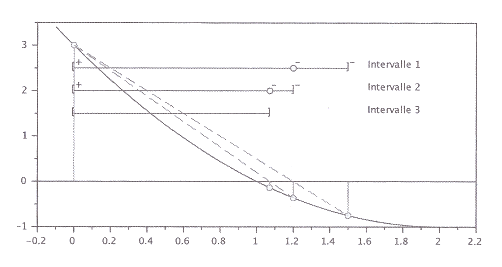
\includegraphics[width=\textwidth]{courbefausseposition}
 \caption{Illustration de la méthode de la fausse position.}
 \label{fig:courbefausseposition}
\end{figure}

\begin{enumerate}
 \item En considérant l'intervalle $[a\,;\,b]$ et une fonction $f$, déterminer l'expression de l'abscisse du point d'intersection entre l'axe des abscisses et la droite qui s'appuie sur les points de la courbe étudiée d'abscisses $a$ et $b$.
 
 \item On se place dans le cas d'une fonction quelconque, qui n'est pas nécessairement convexe. Écrire en python le code d'une fonction permettant de mettre en œuvre la méthode de la fausse position grâce à un algorithme dérivé de la méthode de dichotomie.
\end{enumerate}

\end{document}